% A book summary template inspired by Jan Küster's Left Sidebar CV / https://github.com/jankapunkt/latexcv

\documentclass[11pt,a4paper]{ctexart}	
\usepackage[utf8]{inputenc}	
\usepackage{pdfpages}

% some tex-live fonts - choose your own

%\usepackage[defaultsans]{droidsans}
%\usepackage[default]{comfortaa}
%\usepackage{cmbright}
\usepackage[default]{raleway}
%\usepackage{fetamont}
%\usepackage[default]{gillius}
%\usepackage[light,math]{iwona}
%\usepackage[thin]{roboto}

% set font default
\renewcommand*\familydefault{\sfdefault} 	
\usepackage[T1]{fontenc}

\usepackage{moresize}
\usepackage{fontawesome}

\usepackage{paracol}
\usepackage[margin=1.5cm]{geometry}

\usepackage{fancyhdr}
\pagestyle{empty}
\setlength{\parindent}{0mm}
\usepackage{graphicx}
	
\usepackage{tikz}				
\usetikzlibrary{shapes, backgrounds,mindmap, trees}

\usepackage{transparent}
\usepackage{color}

\definecolor{maincol}{RGB}{ 225, 0, 0 }
\definecolor{darkcol}{RGB}{ 70, 70, 70 }
\definecolor{lightcol}{RGB}{245,245,245}

\usepackage{enumitem}
\setitemize{label={\color{maincol}\faCheck}}

\usepackage[hidelinks]{hyperref}
% A book summary template inspired by Jan Küster's Left Sidebar CV / https://github.com/jankapunkt/latexcv
% The following are the elements taken from said template, albeit from heading onwards was modified and made simpler or added as entirely new elements.



% use to vertically center content
% credits to: http://tex.stackexchange.com/questions/7219/how-to-vertically-center-two-images-next-to-each-other
\newcommand{\vcenteredinclude}[1]{\begingroup
\setbox0=\hbox{\includegraphics{#1}}%
\parbox{\wd0}{\box0}\endgroup}

% use to vertically center content
% credits to: http://tex.stackexchange.com/questions/7219/how-to-vertically-center-two-images-next-to-each-other
\newcommand*{\vcenteredhbox}[1]{\begingroup
\setbox0=\hbox{#1}\parbox{\wd0}{\box0}\endgroup}

% icon shortcut
\newcommand{\icon}[3] { 							
	\makebox(#2, #2){\textcolor{maincol}{\csname fa#1\endcsname}}
}	

% icon with text shortcut
\newcommand{\icontext}[4]{ 						
	\vcenteredhbox{\icon{#1}{#2}{#3}}  \hspace{2pt}  \parbox{0.9\textwidth}{\textcolor{#4}{#3}}
}

% icon with website url
\newcommand{\iconhref}[5]{ 						
    \vcenteredhbox{\icon{#1}{#2}{#5}}  \hspace{2pt} \href{#4}{\textcolor{#5}{#3}}
}

% icon with email link
\newcommand{\iconemail}[5]{ 						
    \vcenteredhbox{\icon{#1}{#2}{#5}}  \hspace{2pt} \href{mailto:#4}{\textcolor{#5}{#3}}
}

%---------------------------------------------------------
% MODIFIED from Kuester's CV
%---------------------------------------------------------
% Renders a a CV section headline with a nice underline in main color.
% param 1: section title
\newcommand{\heading}[1] {
	\vspace{15pt}
	%{\bf\LARGE\color{darkcol}\uppercase{#1}}\\[-4pt]
	{\bf\large{#1}}\\[-4pt]
	{\color{maincol}\rule{0.1\textwidth}{2pt} }\vspace{2pt}
}

%---------------------------------------------------------
% New 
%----------------------------------------------------------
\newcommand{\titlebox}[3]
{\fcolorbox{#1}{#2}{\begin{minipage}[c][4.5cm][c]{\linewidth}%
\begin{center}\large\color{white} #3 %
\end{center}\end{minipage}\\[14pt]
\vspace{-12pt}
}
}

\newcommand{\bigfont}[1]{%
%{\bf\huge\uppercase{#1} } \\[4pt]%
{\bf\huge{#1} } \\[4pt]%
\rule{0.1\textwidth}{1.25pt} \\[4pt]%
}

\newcommand{\titletext}[1]{%
#1 \\[4pt] %
\rule{0.1\textwidth}{1.25pt} \\[4pt]%
}

\renewenvironment{quote}
               {\list{\Large\color{black!50}\faQuoteLeft\phantom{ }}{\rightmargin\leftmargin}%
                \item\relax\Large\color{black!50}\ignorespaces}
               {\unskip\unskip\phantom{xx}\color{black!50}\faQuoteRight\normalsize\endlist}
           





%============================================================================%
\begin{document}

\columnratio{0.8}
\setlength{\columnsep}{2.2em}
\setlength{\columnseprule}{0.2pt}
\colseprulecolor{darkcol}
\begin{paracol}{2}

%\includegraphics[width=\linewidth]{bookcover.jpg}


%\begin{figure}[h]
%    \centering
%    \includegraphics[width=\linewidth]{figure1.jpg}
    %\caption{Graph illustrating how far you can go with the same amount of energy if invested deliberately in just one thing versus diffusion}
%    \label{fig:my_label}
%\end{figure}





\normalsize


% \titlebox{white}{darkcol}{
% \bigfont{数分习题课讲义}

% \titletext{第01章 引论}

% }
% \vspace{1em}

%---------------------------------------------------------------------------------------
\heading{第一章 ~~方程的导出和定解条件}

%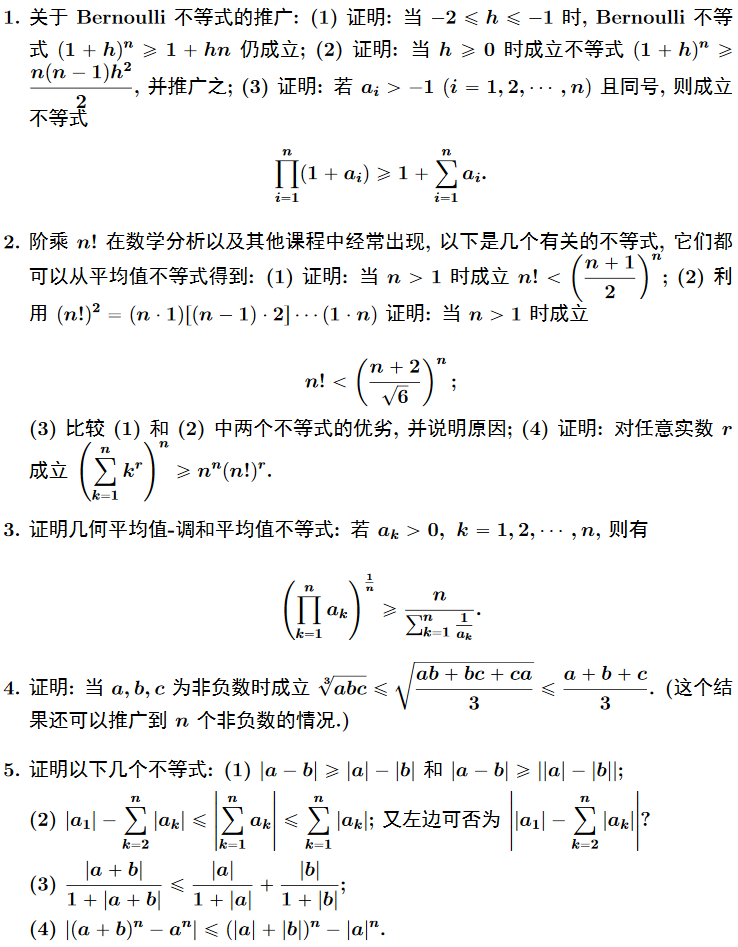
\includegraphics[width=\linewidth]{figure01.png}
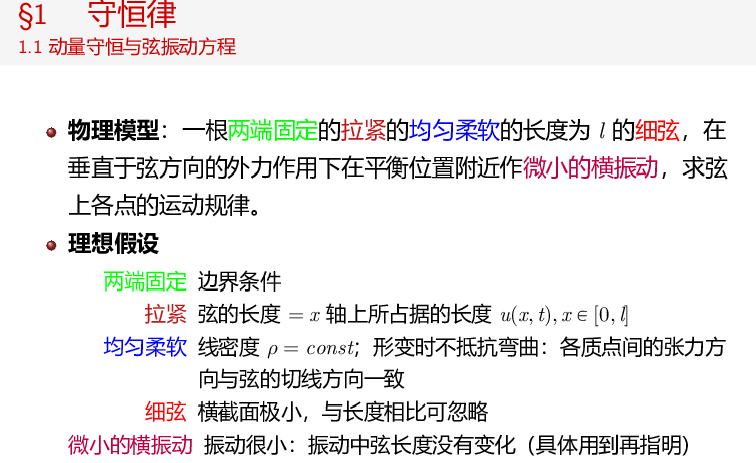
\includegraphics[width=\linewidth]{chap01_09.png}
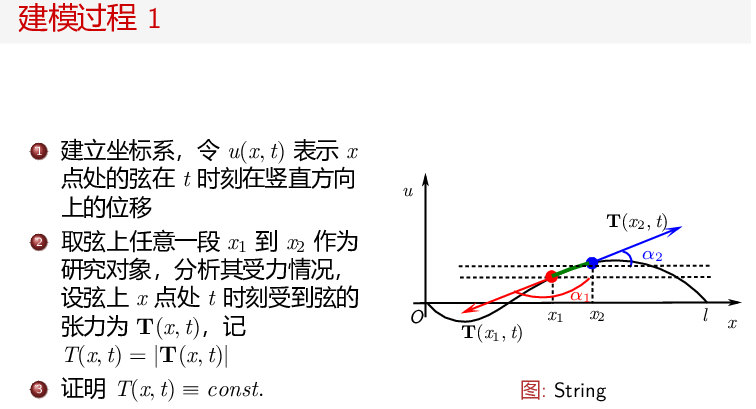
\includegraphics[width=\linewidth]{chap01_10.png}
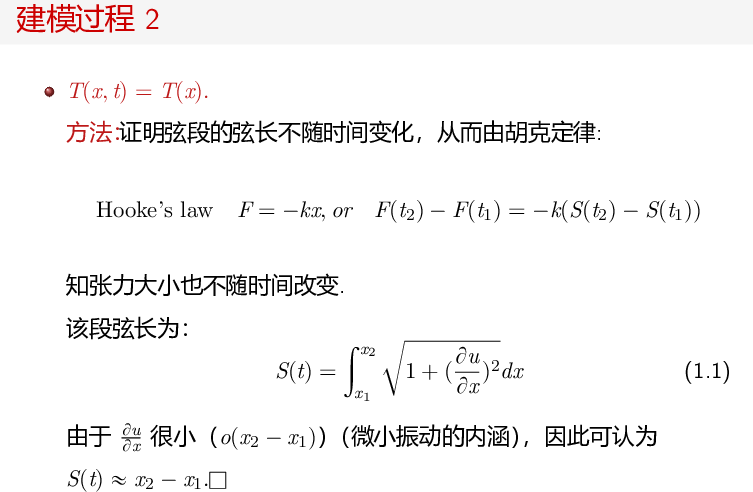
\includegraphics[width=\linewidth]{chap01_11.png}
\newpage
%\heading{2.1.5练习题}
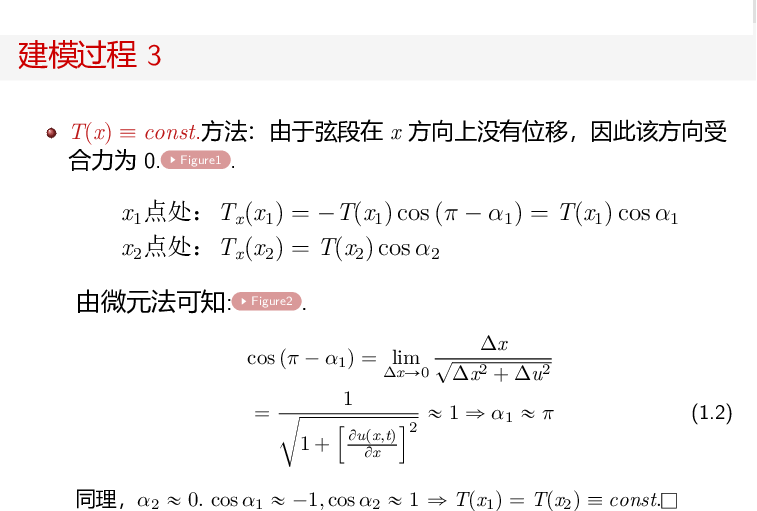
\includegraphics[width=\linewidth]{chap01_12.png}
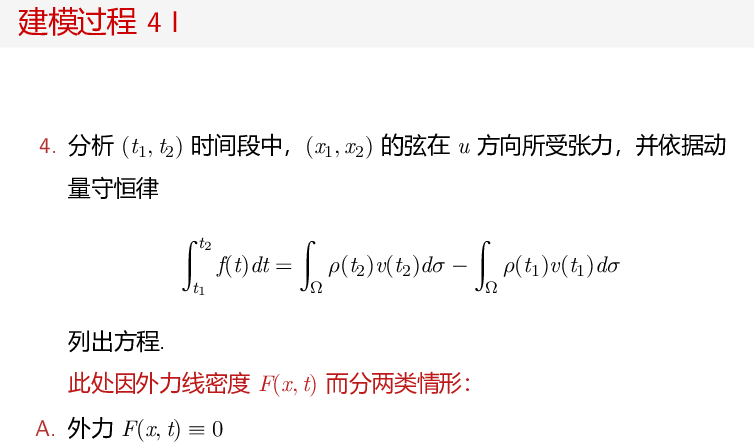
\includegraphics[width=\linewidth]{chap01_13.png}
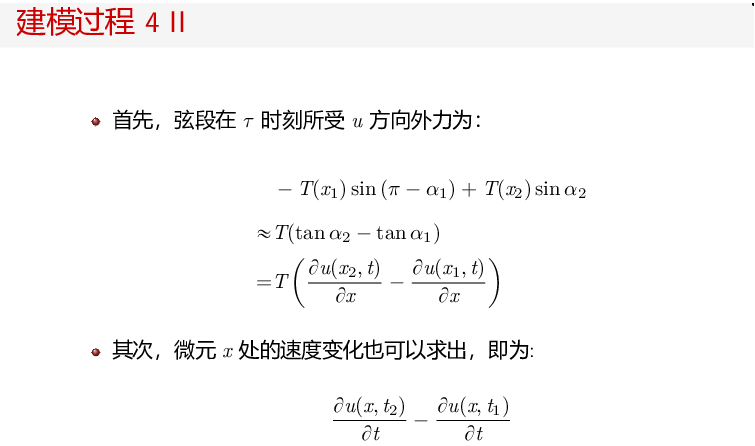
\includegraphics[width=\linewidth]{chap01_14.png}

\newpage
%\heading{2.2.1思考题}

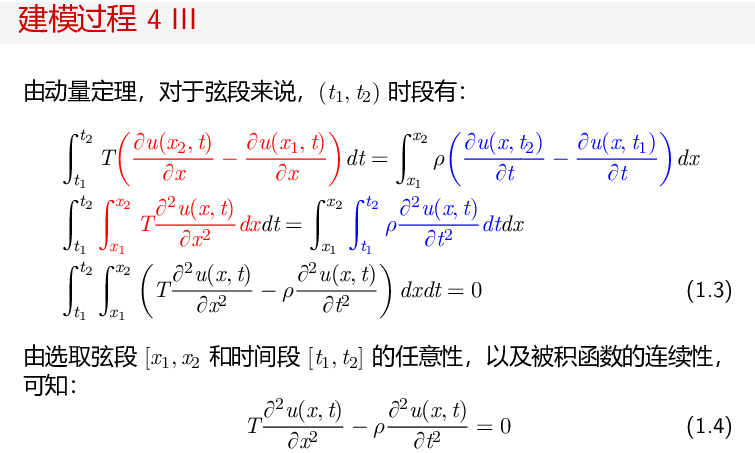
\includegraphics[width=\linewidth]{chap01_15.png}
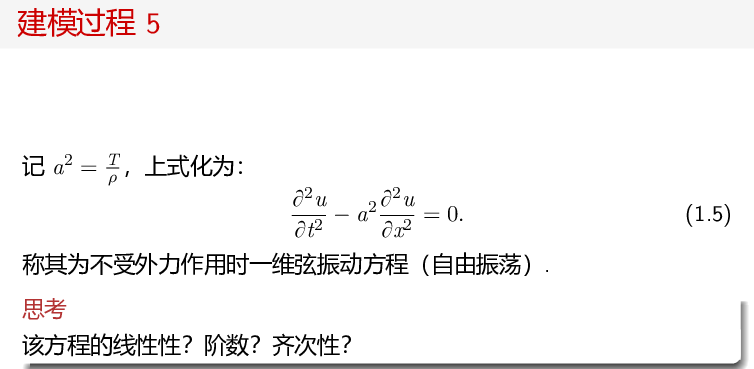
\includegraphics[width=\linewidth]{chap01_16.png}
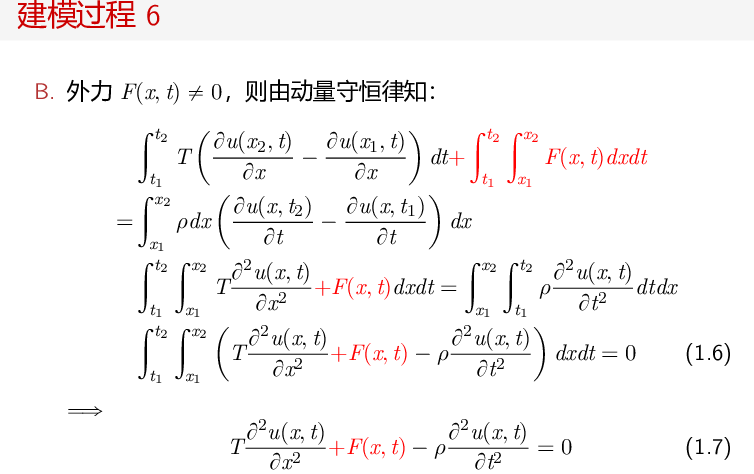
\includegraphics[width=\linewidth]{chap01_17.png}
\newpage
%\heading{2.2.4练习题}

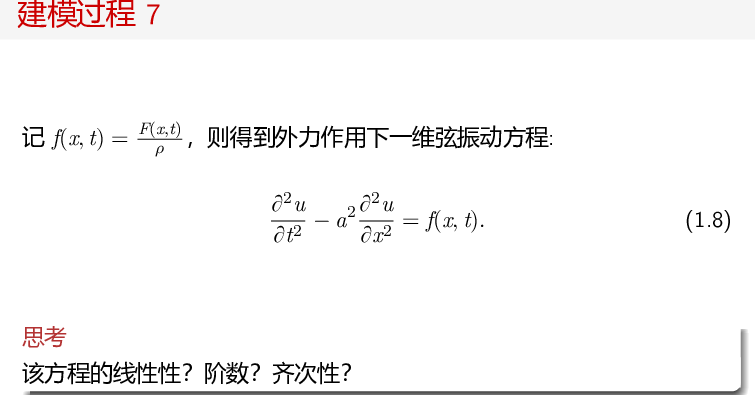
\includegraphics[width=\linewidth]{chap01_18.png}
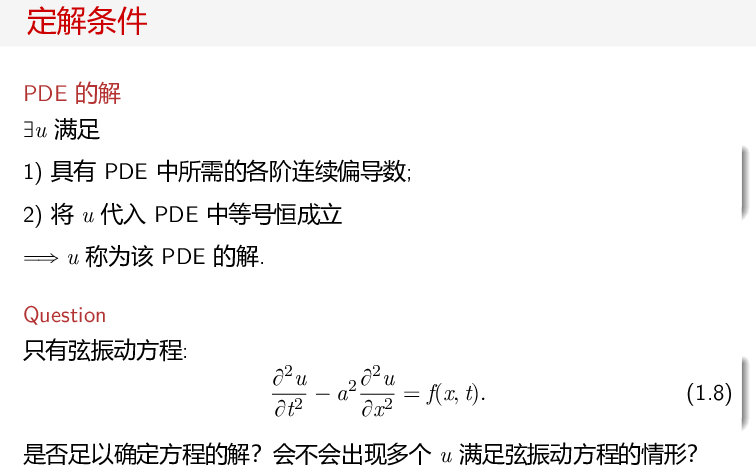
\includegraphics[width=\linewidth]{chap01_19.png}
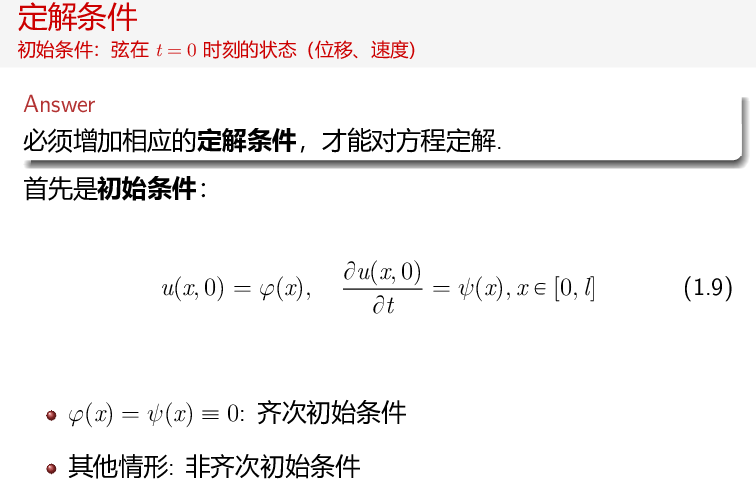
\includegraphics[width=\linewidth]{chap01_20.png}
\newpage
%\heading{2.3.2练习题}

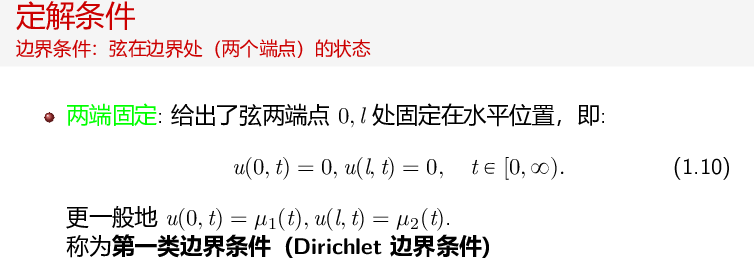
\includegraphics[width=\linewidth]{chap01_21.png}
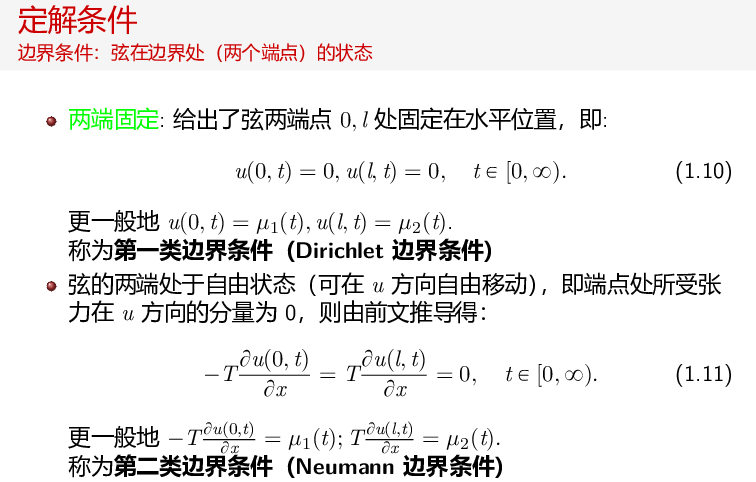
\includegraphics[width=\linewidth]{chap01_22.png}
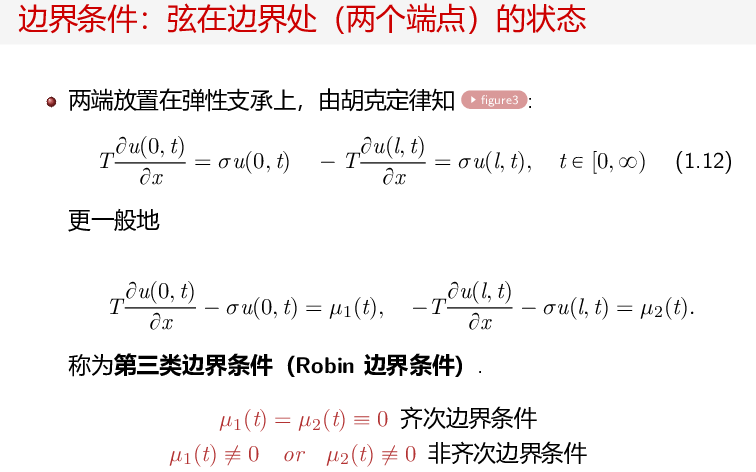
\includegraphics[width=\linewidth]{chap01_23.png}
\newpage
%\heading{2.4.3练习题}

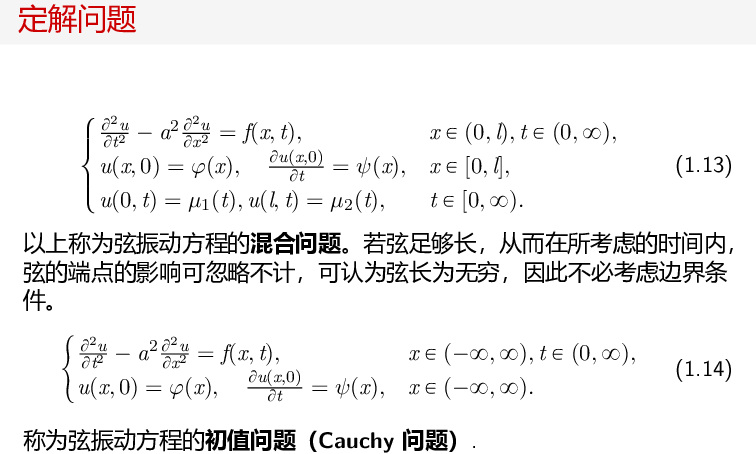
\includegraphics[width=\linewidth]{chap01_24.png}
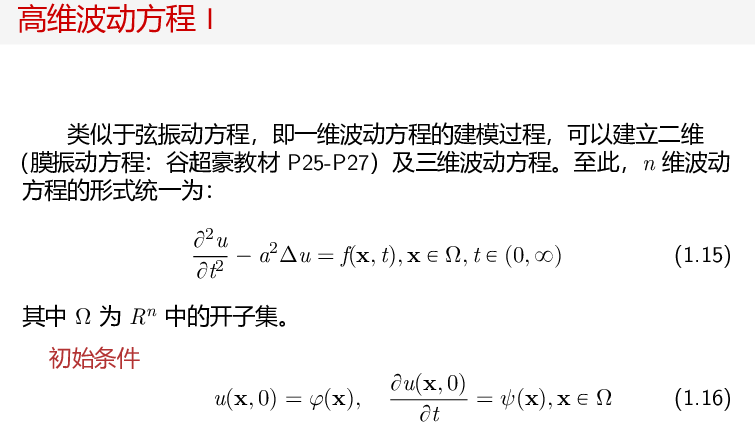
\includegraphics[width=\linewidth]{chap01_25.png}
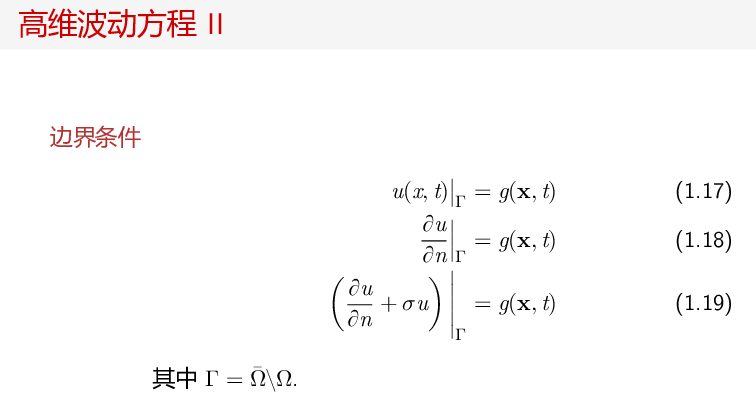
\includegraphics[width=\linewidth]{chap01_26.png}
\newpage
%\heading{2.5.5练习题}

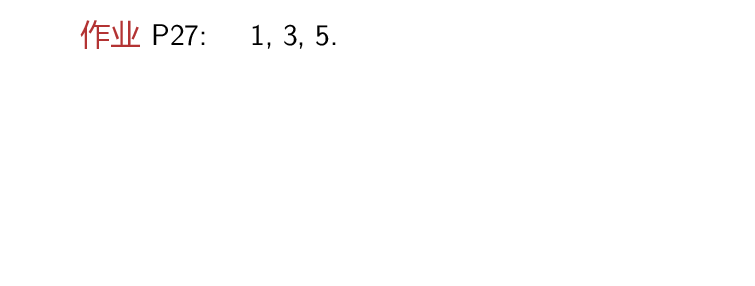
\includegraphics[width=\linewidth]{chap01_27.png}
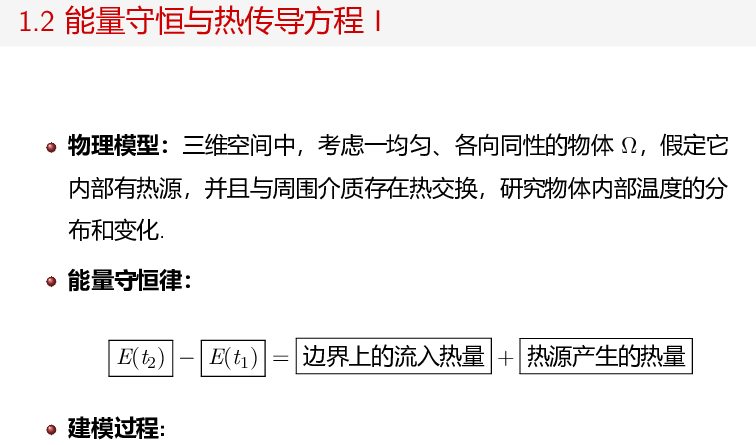
\includegraphics[width=\linewidth]{chap01_28.png}
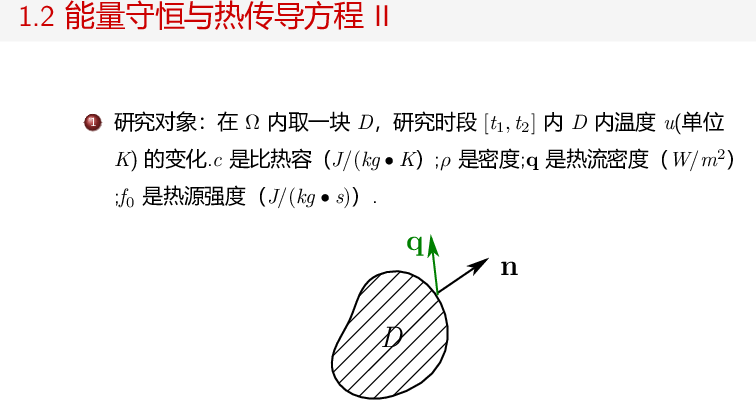
\includegraphics[width=\linewidth]{chap01_29.png}
\newpage
%\heading{2.6.3练习题}

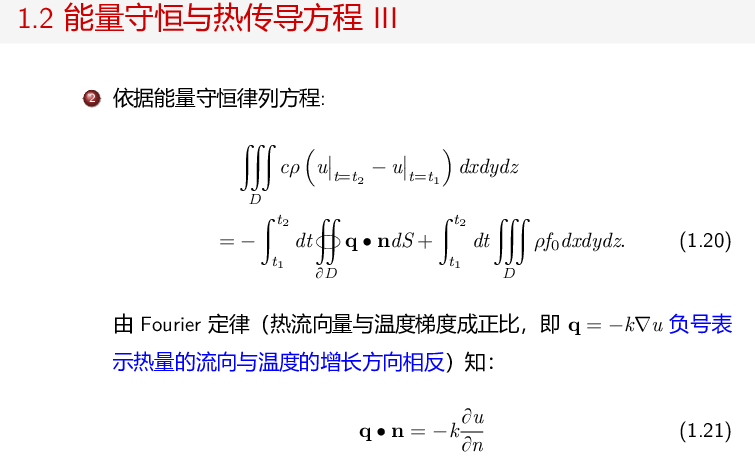
\includegraphics[width=\linewidth]{chap01_30.png}
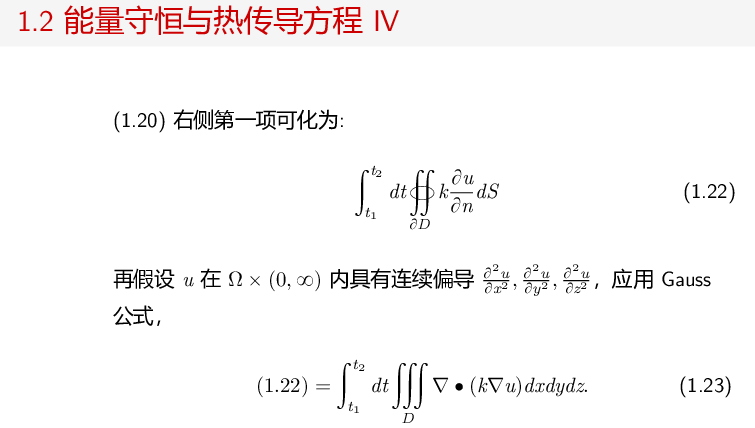
\includegraphics[width=\linewidth]{chap01_31.png}
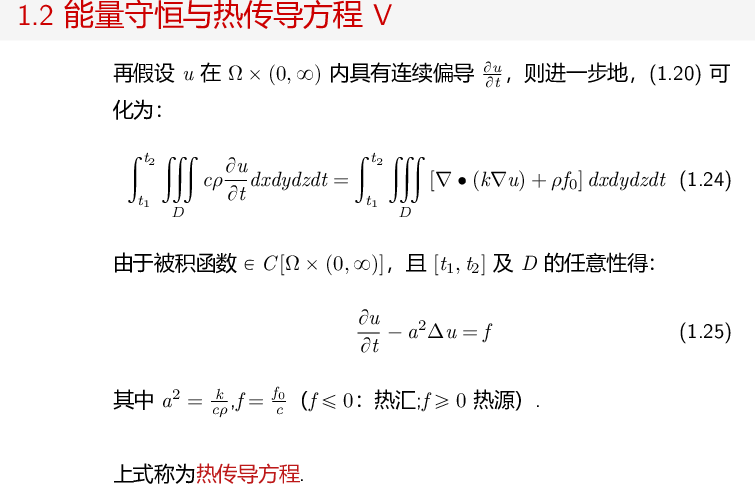
\includegraphics[width=\linewidth]{chap01_32.png}
\newpage
%\heading{2.7.3第1组参考题}

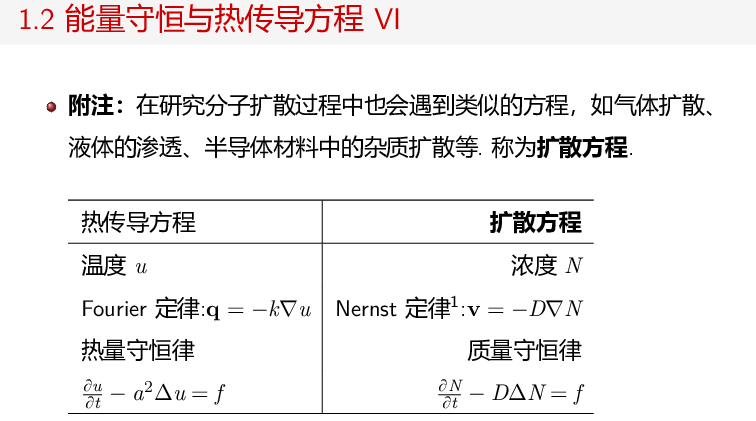
\includegraphics[width=\linewidth]{chap01_33.png}
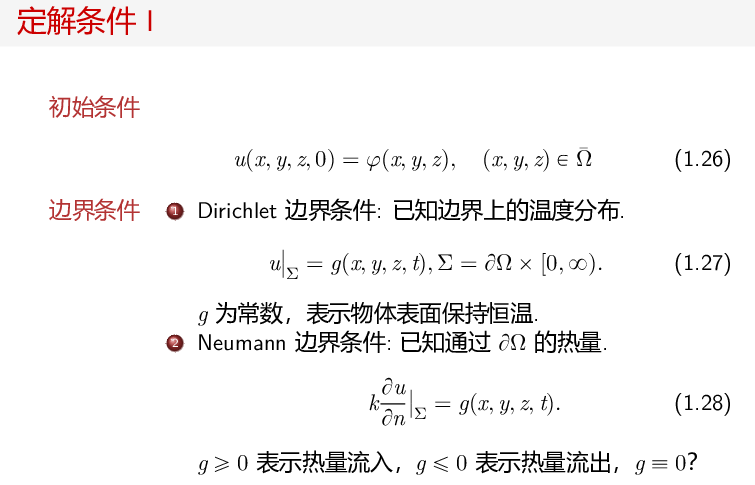
\includegraphics[width=\linewidth]{chap01_34.png}
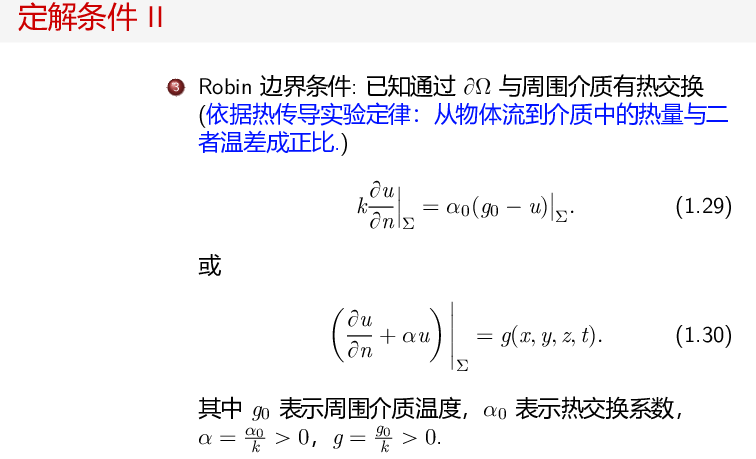
\includegraphics[width=\linewidth]{chap01_35.png}
\newpage
%\heading{2.7.3第1组参考题}

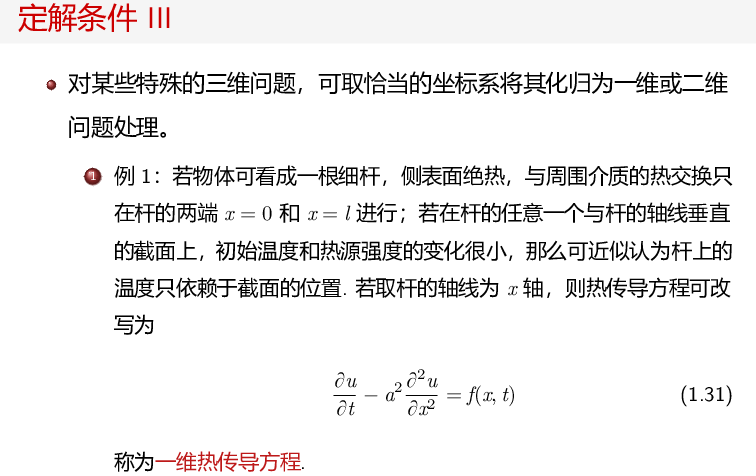
\includegraphics[width=\linewidth]{chap01_36.png}
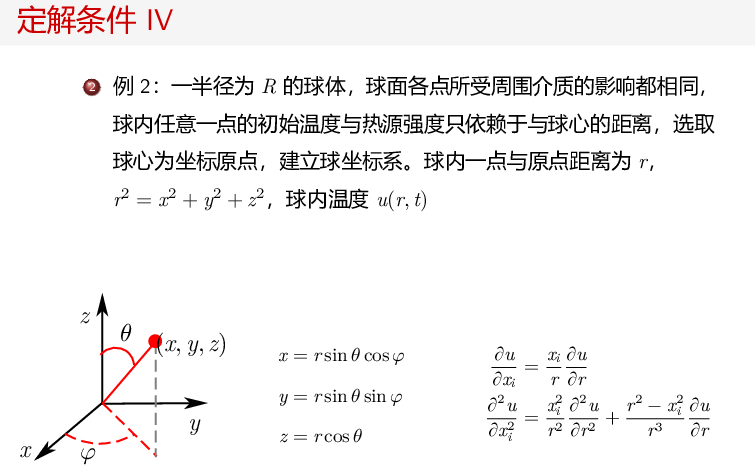
\includegraphics[width=\linewidth]{chap01_37.png}
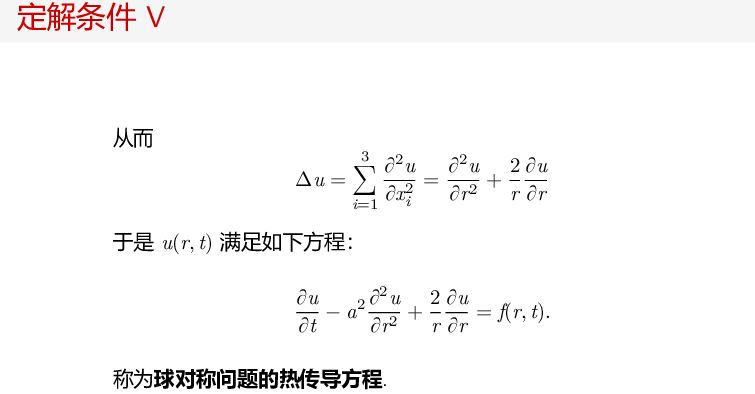
\includegraphics[width=\linewidth]{chap01_38.png}
\newpage

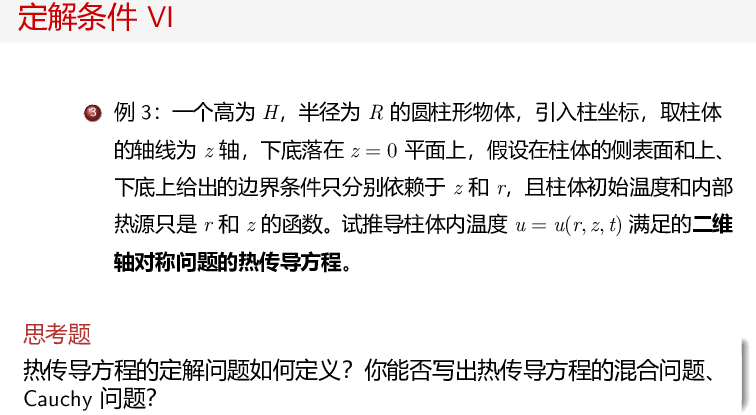
\includegraphics[width=\linewidth]{chap01_39.png}
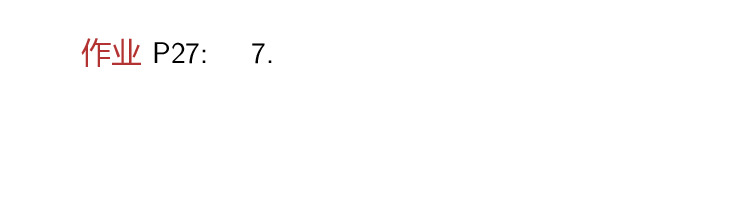
\includegraphics[width=\linewidth]{chap01_40.png}
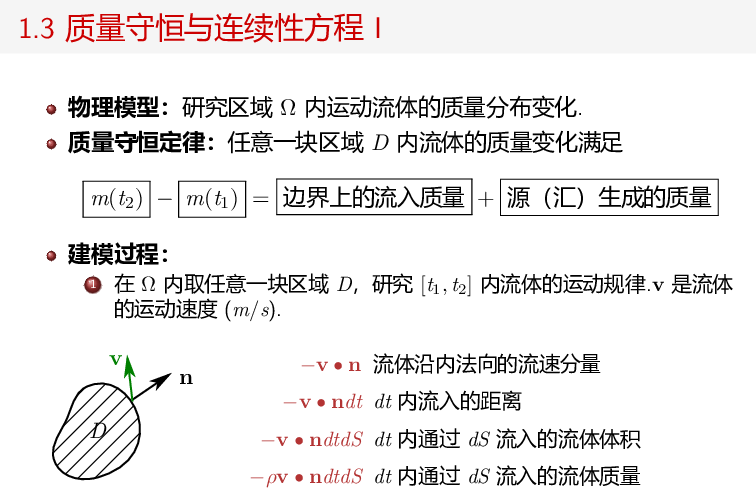
\includegraphics[width=\linewidth]{chap01_41.png}
\newpage

%\heading{2.7.3第2组参考题}

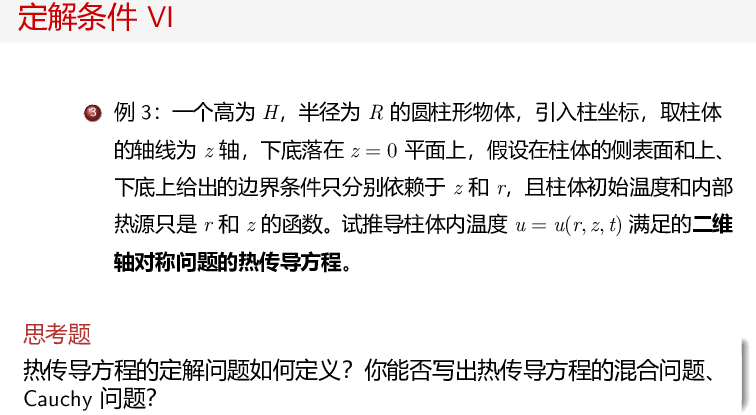
\includegraphics[width=\linewidth]{chap01_39.png}
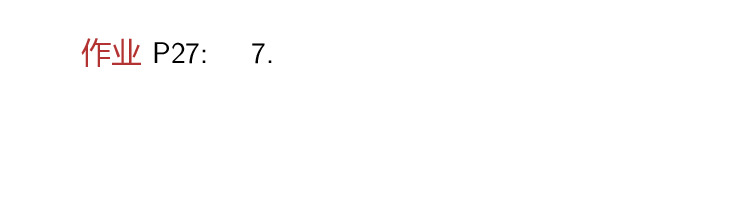
\includegraphics[width=\linewidth]{chap01_40.png}
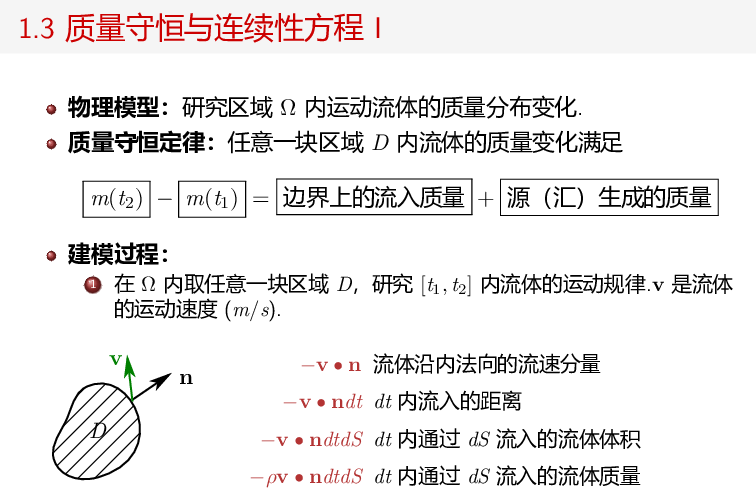
\includegraphics[width=\linewidth]{chap01_41.png}

\newpage
%\heading{2.8第1次习题课}
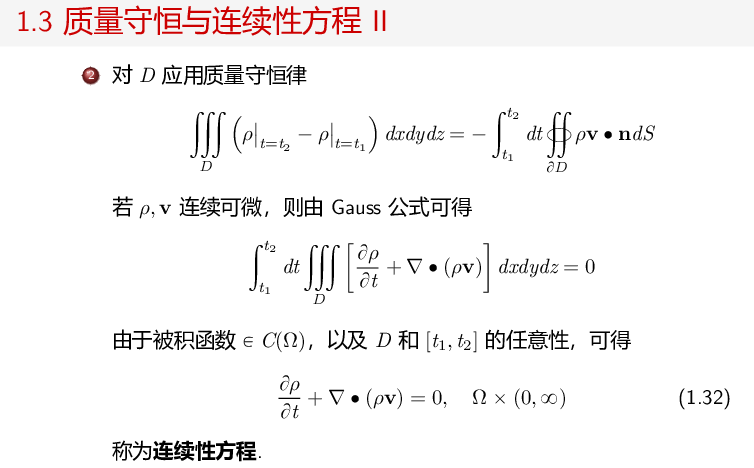
\includegraphics[width=\linewidth]{chap01_42.png}
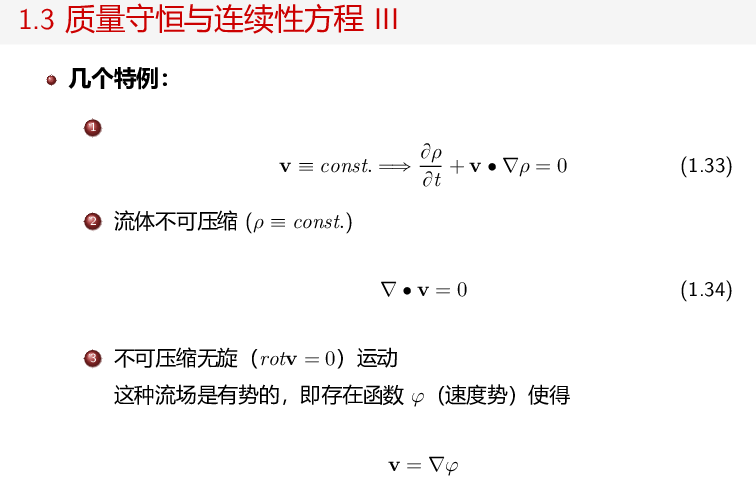
\includegraphics[width=\linewidth]{chap01_43.png}
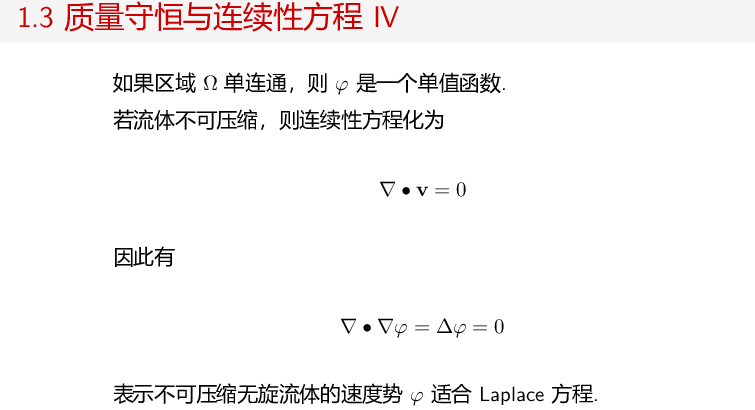
\includegraphics[width=\linewidth]{chap01_44.png}
\newpage
%\heading{2.8第1次习题课}
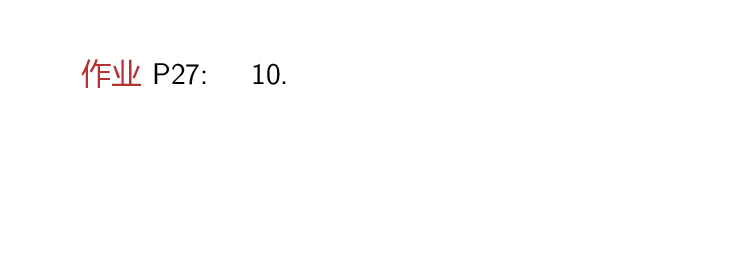
\includegraphics[width=\linewidth]{chap01_45.png}
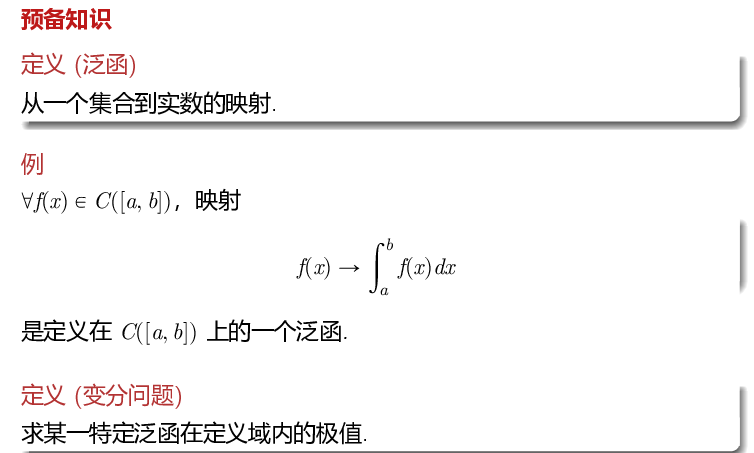
\includegraphics[width=\linewidth]{chap01_46.png}
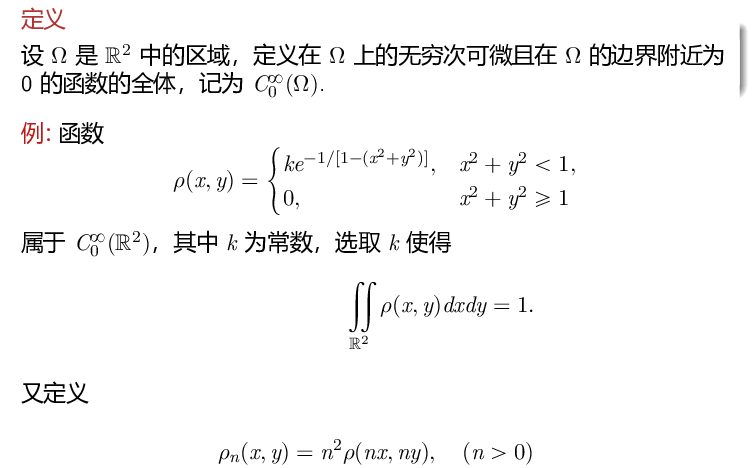
\includegraphics[width=\linewidth]{chap01_47.png}
\newpage
%\heading{2.8第3次习题课}

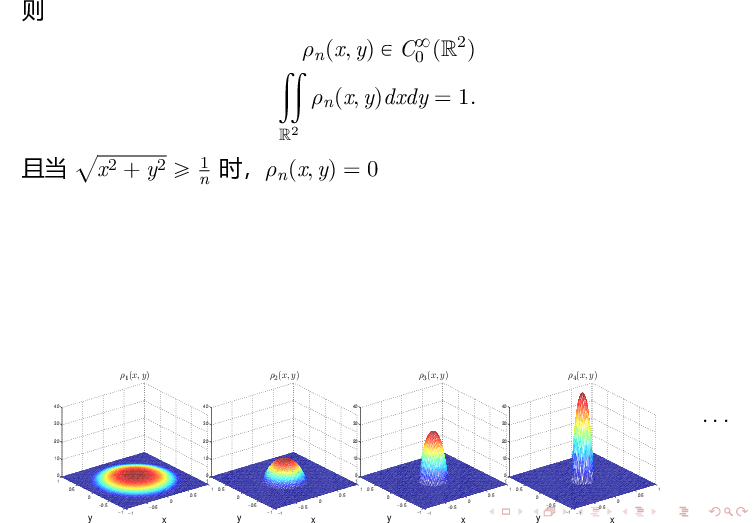
\includegraphics[width=\linewidth]{chap01_48.png}
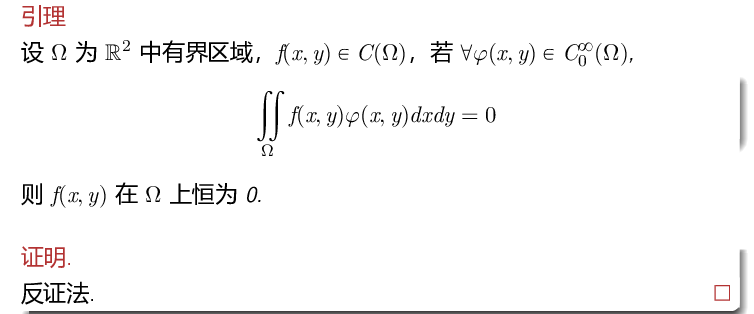
\includegraphics[width=\linewidth]{chap01_49.png}
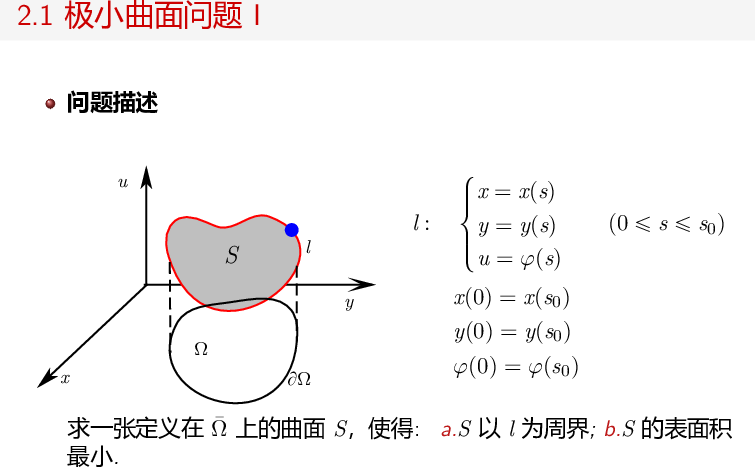
\includegraphics[width=\linewidth]{chap01_50.png}
\newpage
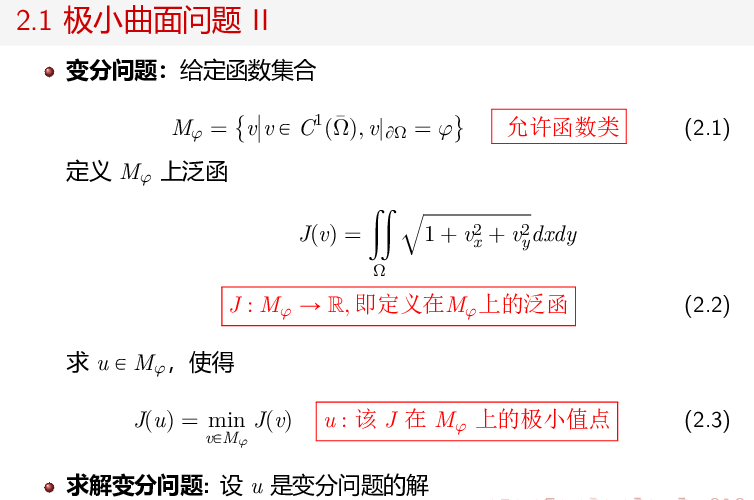
\includegraphics[width=\linewidth]{chap01_51.png}
\includegraphics[width=\linewidth]{chap01_52.png}
\includegraphics[width=\linewidth]{chap01_53.png}
\newpage
\includegraphics[width=\linewidth]{chap01_54.png}
\includegraphics[width=\linewidth]{chap01_55.png}
\includegraphics[width=\linewidth]{chap01_56.png}
\newpage
\includegraphics[width=\linewidth]{chap01_57.png}
\includegraphics[width=\linewidth]{chap01_58.png}
\includegraphics[width=\linewidth]{chap01_59.png}
\newpage
\includegraphics[width=\linewidth]{chap01_60.png}
\includegraphics[width=\linewidth]{chap01_61.png}
\includegraphics[width=\linewidth]{chap01_62.png}
\newpage
\includegraphics[width=\linewidth]{chap01_63.png}
\includegraphics[width=\linewidth]{chap01_64.png}
\includegraphics[width=\linewidth]{chap01_65.png}
\newpage
\includegraphics[width=\linewidth]{chap01_66.png}
\includegraphics[width=\linewidth]{chap01_67.png}
\includegraphics[width=\linewidth]{chap01_68.png}
\newpage
\includegraphics[width=\linewidth]{chap01_69.png}
\includegraphics[width=\linewidth]{chap01_70.png}
\includegraphics[width=\linewidth]{chap01_71.png}
\newpage
\includegraphics[width=\linewidth]{chap01_72.png}
\includegraphics[width=\linewidth]{chap01_73.png}
\includegraphics[width=\linewidth]{chap01_74.png}
\newpage
\includegraphics[width=\linewidth]{chap01_76.png}
\includegraphics[width=\linewidth]{chap01_77.png}
\includegraphics[width=\linewidth]{chap01_79.png}
\newpage
% \begin{figure}[h]
%    \centering
%    \includegraphics[width=\linewidth]{figure01.png}
% \end{figure}

% \begin{figure}[h]
%    \centering
%    \includegraphics[width=\linewidth]{figure02.png}
% \end{figure}

\small
\switchcolumn

\heading{笔记区}
\newpage
\heading{笔记区}
\newpage
\heading{笔记区}
\newpage
\heading{笔记区}
\newpage
\heading{笔记区}
\newpage
\heading{笔记区}
\newpage
\heading{笔记区}
\newpage
\heading{笔记区}
\newpage
\heading{笔记区}
\newpage
\heading{笔记区}
\newpage
\heading{笔记区}
\newpage
\heading{笔记区}
\newpage
\heading{笔记区}
\newpage
\heading{笔记区}
\newpage
\heading{笔记区}
\newpage
\heading{笔记区}
\newpage
\heading{笔记区}
\newpage
\heading{笔记区}
\newpage
\heading{笔记区}
\newpage
\heading{笔记区}
\newpage
\heading{笔记区}
\newpage
\heading{笔记区}
\newpage
\heading{笔记区}
\newpage
\heading{笔记区}
\newpage

\end{paracol}





\end{document}

